\documentclass[conference]{IEEEtran}
\IEEEoverridecommandlockouts
% The preceding line is only needed to identify funding in the first footnote. If that is unneeded, please comment it out.
\usepackage{cite}
\usepackage{amsmath,amssymb,amsfonts}
\usepackage{algorithmic}
\usepackage{caption}
\usepackage{subcaption}
% \usepackage{subfigure}
\usepackage{color}
%\usepackage[dvipdfmx]{graphicx}
\usepackage{graphicx}
% by zhao, in overleaf no need to add [dvipdfmx] for disp eps figure
\usepackage{textcomp}
\usepackage{xcolor}
\usepackage{enumerate}
\usepackage{multirow}
\usepackage{amsmath}
\usepackage{amssymb}
\usepackage[utf8]{inputenc}
\usepackage[ruled]{algorithm2e}
\usepackage[colorinlistoftodos]{todonotes}
\def\BibTeX{{\rm B\kern-.05em{\sc i\kern-.025em b}\kern-.08em
    T\kern-.1667em\lower.7ex\hbox{E}\kern-.125emX}}
% by michiko
\newtheorem{definition}{Definition}
%
\begin{document}
% \title{Optimize Configuration For Mismatched PV System}
\title{A Rapid Feasibility Checking for Reconfiguration of Mismatched PV Arrays}
\author{\IEEEauthorblockN{Dafang Zhao, Fukuhito Ooshita, and Michiko Inoue}
%Email: 
\IEEEauthorblockA{Nara Institute of Science and Technology, Japan\\
Email:   \{zhao.dafang.yu7, f-ooshita, kounoe\}@is.naist.jp}}
\maketitle

\begin{abstract}
Power generation efficiency of Photovoltaic (PV) arrays is significantly affected by partial shading and PV cell damage. Partial shading or PV cell damage induces mismatched power generation among PV panels and causes the efficiency loss of power generation. Power generation of mismatched PV arrays can be recovered by re-configuring connection of PV panels. Recently, an efficient and effective reconfiguration method is proposed where it first selects candidates of configurations with approximation and then find the best one with precise power simulation. However, we found that some of  configuration candidates are not able to be realized and the method does not show any systematic way to identify such a feasibility. In this paper, we propose an algorithm to rapidly check feasibility that a given configuration candidate can be actually formed by given PV panels. The experimental results demonstrate that the proposed method rapidly checks the feasibility with a small error rate \textcolor{blue}{(this part will be written with actual values)}.
\end{abstract}

% \begin{IEEEkeywords}
% component, formatting, style, styling, insert
% \end{IEEEkeywords}

\section{Introduction}
As fossil fuel depletion and environmental pollution become more serious, green and renewable energy has become necessary for a sustainable society and environment. Photovoltaic (PV) systems receive significant attention since the sun has unlimited energy and PV arrays can be easily scaled up. However, due to the nature of a PV cell, which is a basic component of a PV array, PV arrays are sensitive to partial shading and PV cell damage. PV cells could not uniformly generate power when PV cells experience different irradiances or some of cells have physical defects, and such a mismatched condition might accelerate heating and aging of PV cells and cause further damaging. To prevent PV cells from damaging, bypass diodes are usually placed in PV arrays and they are turned on in mismatched conditions. However, it causes a significant loss of power generation. 

PV arrays are hierarchically constructed such that a group of PV cells form a PV module, a group of PV modules form a PV panel, and a group of PV panels form a PV array. Power generation of mismatched PV arrays can be recovered by reconfiguring connection of these components. 
Fig.\ref{compare} shows an example of power generations of a PV array with a partial shading. We distributed shading cells non-uniformly to a PV array with 
3 $\times$ 4 PV panels
% \textcolor{blue}{$? \times ?$ PV panels} 
and applied power simulation. Before reconfiguration, it has four peaks in power generation, while, if we reconfigure connection among PV panels, it can generate more power. 


Though several reconfiguration methods have been proposed, most works consider reconfiguration in PV cell or PV module level \cite{nguyen2008adaptive,wang2014architecture,storey2013improved,storey2014optimized,udenze2018reconfiguration}. 
However, cell level reconfiguration requires a significantly high computation time and a large number of switches for reconfiguration. In addition, they require a special PV panels with capability of switching, and cannot be applied to the system constructed with standard PV panels. From a practical view, reconfiguration of connection among PV panels is a realistic solution since a PV panel is manufactured as a physical one panel with two terminals and PV panels can be flexibly interconnected. 

% finding global maximum point tracking (without reconfiguration) 
% and reconfigured PV array.
%It puts into evidence that after reconfiguration shadowed PV array be able to generate more power and P—V curve has only one peak which is very useful for maximum point tracking devices.
\begin{figure}[t]
    \centering
    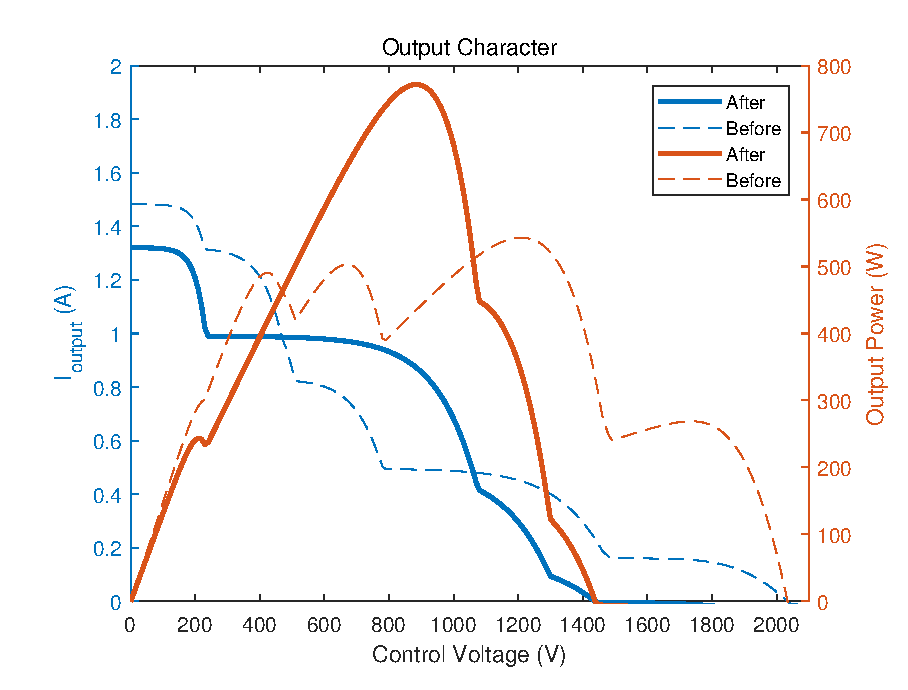
\includegraphics[width=0.8\linewidth]{fig/new_compare.eps}
    \caption{Power generation before and after reconfiguration}
    \label{compare}
\end{figure}

Reconfiguration in PV panel level has been investigated\cite{carotenuto2015evolutionary,hu2017non,orozco2016optimized}. 
A PV array reconfiguration using genetic algorithm (GA) was proposed in \cite{carotenuto2015evolutionary}. Though it can give a new configuration, computing cost is significantly high and the algorithm cannot generate the best configuration precisely.  
Hu et al. also addressed PV panel reconfiguration where they formulate a nonlinear integer programming problem to optimize power generation by reconfiguration \cite{hu2017non}.
%An algorithm based on particle swarm optimization to find switch matrix topology is proposed \cite{iraji2017optimisation}. 
Orozco-Gutierrez et al. proposed an efficient and effective reconfiguration method\cite{orozco2016optimized} where it first selects candidates of configurations with approximation and then finds the best one with precise power simulation. However, the candidates are specified in a PV module level though PV modules could not be fully reconfigured. Actually, we found that some of configuration candidates are not able to be realized. However, the paper\cite{orozco2016optimized}  does not show any systematic way to identify such a feasibility. 

In this paper, we propose an algorithm to rapidly check feasibility that a given configuration candidate is actually formed by given PV panels. The proposed method can efficiently check the feasibility while identifying most feasible cases accurately. The experimental results demonstrate the effectiveness of the proposed method where ...

The remaining of this paper is organized as follows. Section \ref{Sec2} introduces a PV array which is a targeting PV system in this paper. Section \ref{Sec3} gives related works. Section \ref{Sec4} defines a feasibility, and Sections \ref{Sec5} and \ref{Sec6} give the details of algorithm and evaluation. Section \ref{Sec7} shows the experimental results. Conclusions are provided in the last section.

\section{Photovoltaic array}\label{Sec2}
A PV system or PV array is composed of PV panels that have two terminals of plus and minus and can be interconnected. There are two common connection styles for PV arrays, \textit{series-parallel} array and \textit{total-cross-tied} array. 
In a series-parallel array, PV panels are connected in series, and multiple series connections are connected in parallel. In a total-cross-tied array, parallel connections of PV panels are connected in series. In this paper, we focus on series-parallel arrays, however the basic idea of the proposed method can be applied also to total-cross-tied arrays. Hereafter, we simply call a series-parallel array a \textit{PV array}. 

Figure \ref{model} shows an example of a PV array. A PV array is a parallel connection of (PV) strings where a string is a series connection of PV panels. A PV panel is a series connection of PV modules, and a PV module is a parallel connection of a series of PV cells and a bypass diode. A typical PV panel is composed of three PV modules each of which has 12-24 PV cells. A PV module can generate power for a given voltage according to its I-V characteristics as shown in Fig.\ref{fig:IV}(a). The I-V characteristics is affected by irradiance level and physical damage of PV cells. Figure \ref{fig:IV}(a) also shows a typical degradation of a I-V characteristics where generated current is reduced with some ratio while keeping the voltage range. When a PV panel has a partial shade, that is its PV modules have different irradiance levels and hence different I-V characteristics, the PV panels might have multiple peaks (maximum power points, MPPs) in power generation as shown in Fig.\ref{fig:IV}(b). 

To find out accurate I-V characteristics of a PV panel, we need a time consuming power simulation. However, we can roughly understand I-V characteristics of a PV panel (and also a string) as follows. When a control voltage is low, PV modules with high irradiance level are active while PV modules with low irradiance level are inactive with turning on their bypass diodes. In this case, a high current can flow in the PV panel. When control voltage is high, some of bypass diodes become turning off and the corresponding PV modules become active. In this case, the current level is reduced and generated power sometimes increases and sometimes decreases. The generated power at MPPs can be roughly estimated. In Fig.\ref{fig:IV}(b), one PV panel has three PV modules with different irradiance levels. The peak currents for these modules are 5A, 3A, and 1.5A, respectively. Voltages at MPPs are roughly 20V, 40V, 60V in Fig.\ref{fig:IV}(b), those are roughly multiples of a voltage of MPP for one PV module (around 20V in this case). At the first MPP (MPP1), only one PV module with a peak current of 5A is active at a control voltage of 20V, so the generated power is 100W. At the second MPP (MPP2), two PV modules with peak currents of 5A and 3A are active at a control voltage of 40V. In this case, the current level of the PV panel is 3A since two PV panels are connected in series and they have to have the same current level, and the generated power is 120W. At the third MPP (MPP3), the current level of the PV panel is 1.5A at a control voltage of 60V, and the generated power is 90W. 

In a PV array, we have two constraints. PV panels in the same string have the same current level, while all the strings have the same control voltage. When considering reconfiguration of PV panel connection, we should find out the best configuration while considering these constraints. 

\begin{figure}[t]
    \centering
    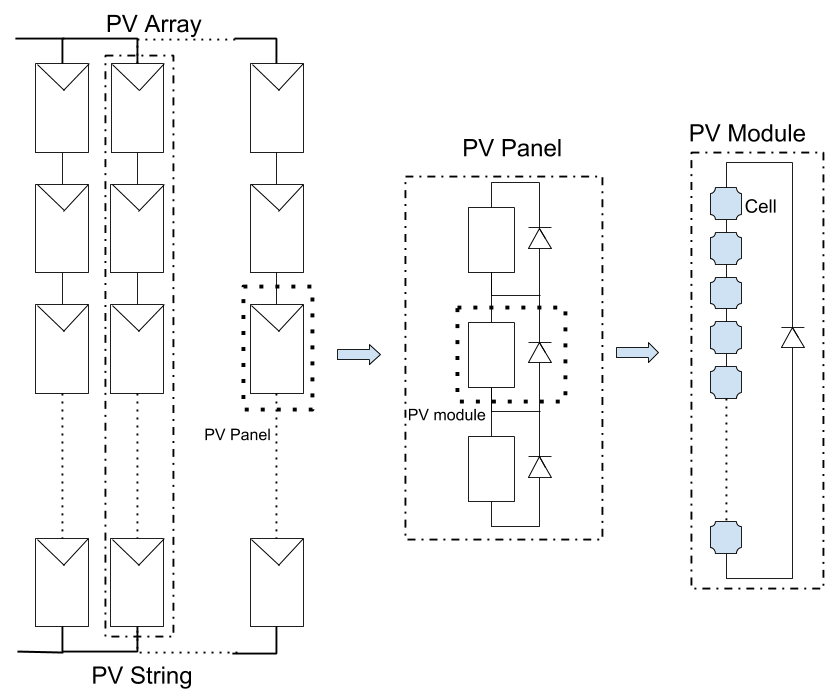
\includegraphics[width=0.8\linewidth]{module.png}
    \caption{PV array, string, module and panel}
    \label{model}
\end{figure}

\begin{figure}
     \centering
    \begin{subfigure}[b]{0.5\linewidth}
        \centering
        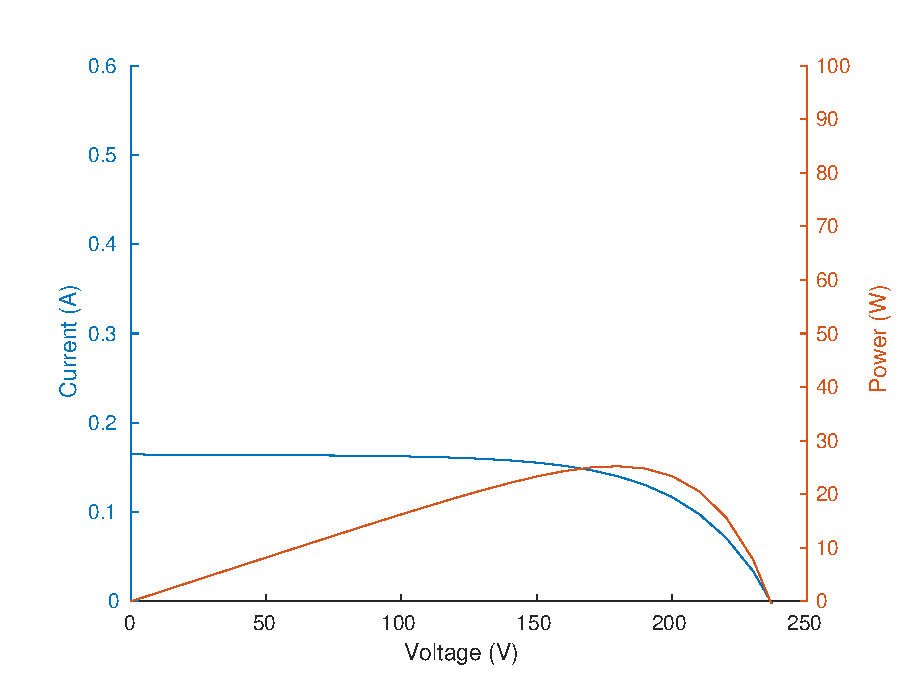
\includegraphics[width=\linewidth]{fig/Module_1.eps}
        \caption{PV module 1}
     \end{subfigure}
     \begin{subfigure}[b]{0.5\linewidth}
        \centering
        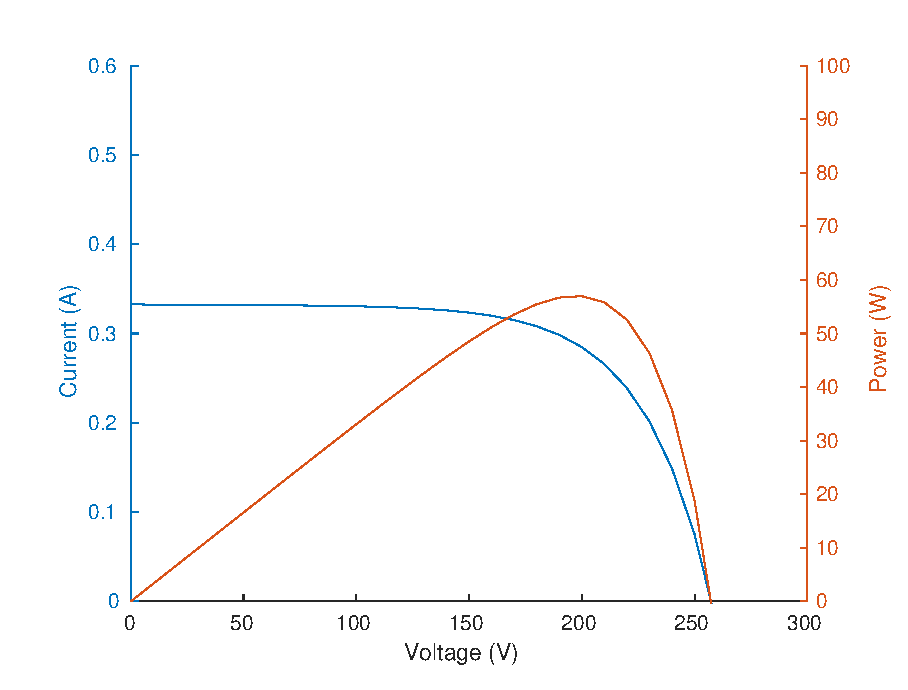
\includegraphics[width=\linewidth]{fig/Module_2.eps}
        \caption{PV module 2}
     \end{subfigure}
     \begin{subfigure}[b]{0.5\linewidth}
        \centering
        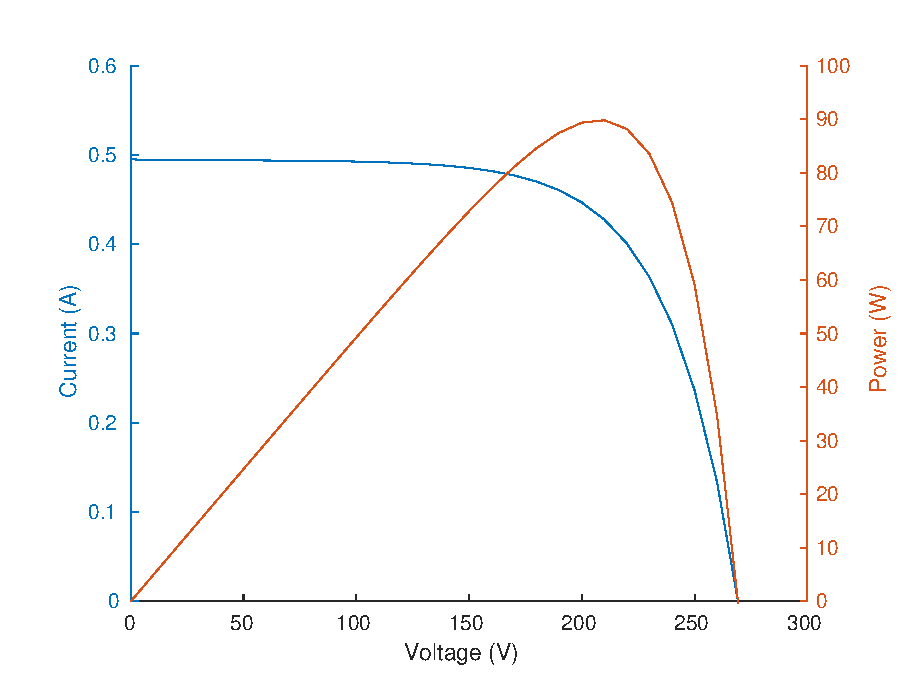
\includegraphics[width=\linewidth]{fig/Module_3.eps}
        \caption{PV module 3}
    \end{subfigure}
    \hfill
    \begin{subfigure}[b]{0.9\linewidth}
        \centering
        \vspace{3mm}
        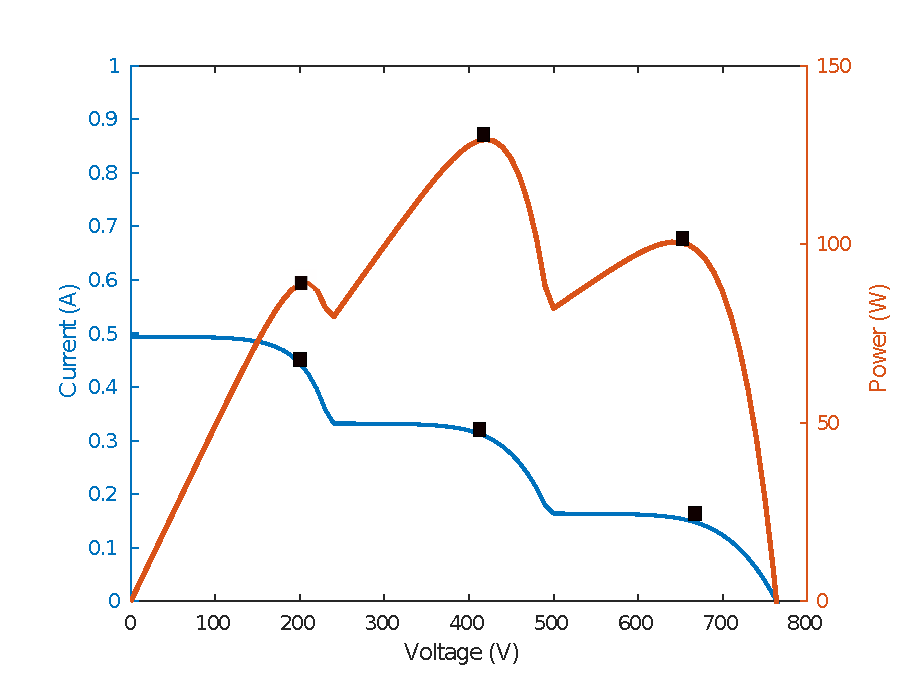
\includegraphics[width=\linewidth]{fig/pv_panel_edit.eps}
        \caption{PV panel}
    \end{subfigure}
    \caption{I-V characteristics}
    \label{fig:IV}
\end{figure}

%In this paper we use the following model of PV array, module, string and panel as showed in Fig.\ref{model}. In general, a PV array is a combination of multiple PV panels. Several series-connected PV panels in formed of a string. And several parallel connected string in formed of PV array. This is typical S-P network PV array. A PV panel usually formed by three series-connected PV module which in formed of several series-connected PV cells. For each PV module a bypass diode is connected in parallel for reversing the reverse current. PV cells in a PV panel may have different conditions (irradiance or fault) and hence have different  upper limits for their generated currents. Therefore, as shown in Fig.\ref{one_panel} for lower control voltage, only PV cells can generate high currents be able to work and other PV cells don't generate current with their bypass diode turned on. Fig.\ref{ser-par} show I-V character for two series and parallel connected PV panels. The series-connection structure accepts a wider range of control voltage and parallel-connection structure can generate higher current.


%When understanding the I-V characteristics of different structure of PV panels, by using the algorithm in \cite{carotenuto2014online} we can find the I-V curves of panels and (near) MPPs, short circuit current, open circuit voltage of each panel in mismatch condition. These values form a fingerprint of connection.
%\begin{figure}
%     \centering
%     \begin{subfigure}[b]{0.8\linewidth}
%         \centering
 %        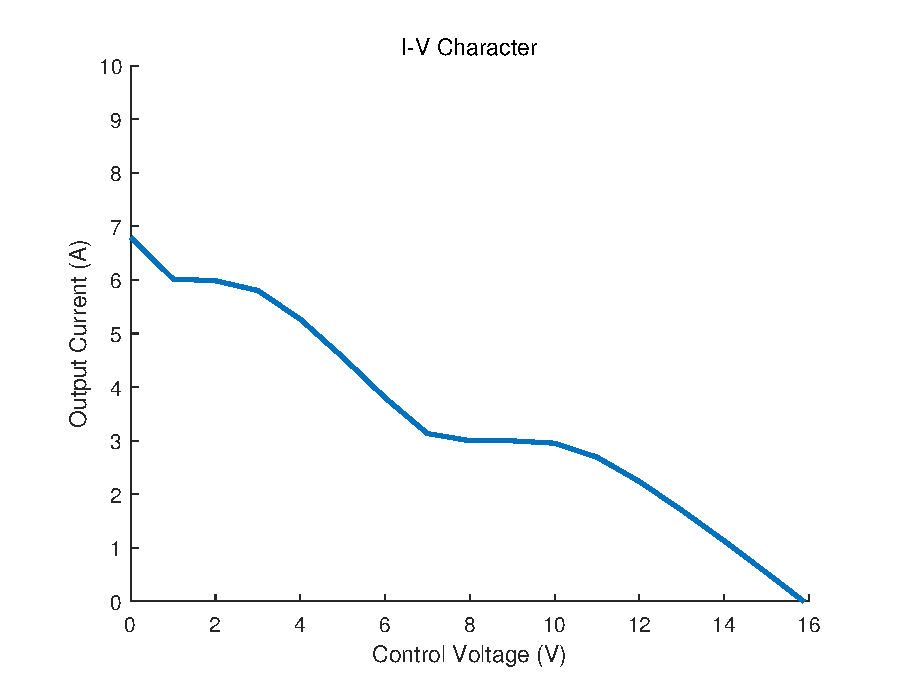
\includegraphics[width=\linewidth]{one-panel.eps}
 %        \caption{I-V characteristics on different control voltage}
 %        \label{one_panel}
 %    \end{subfigure}
%     \hfill
%     \begin{subfigure}[b]{0.8\linewidth}
 %        \centering
 %        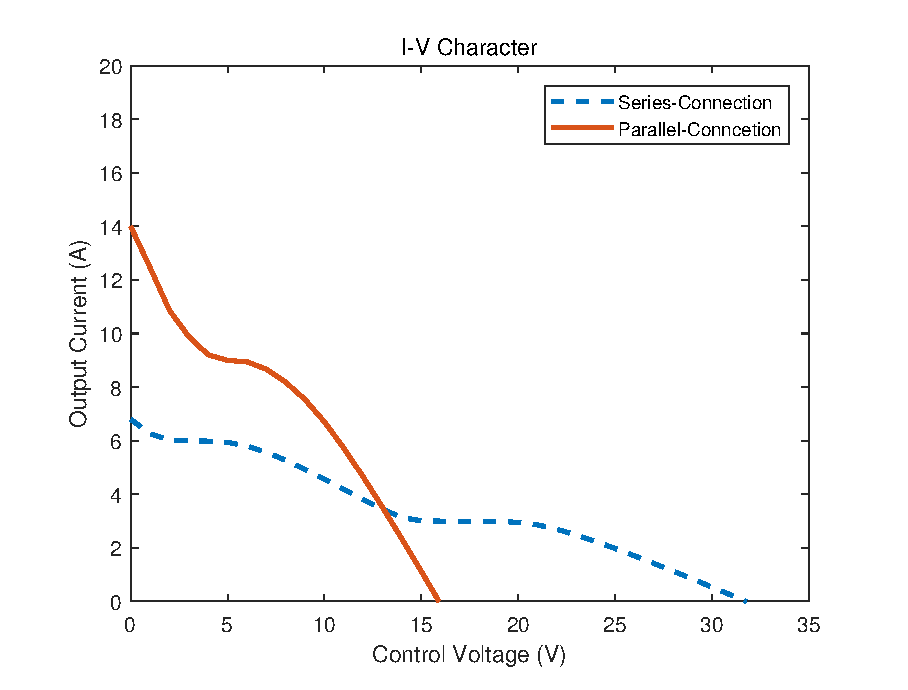
\includegraphics[width=\linewidth]{ser-par.eps}
 %        \caption{Series and parallel connection I-V character}
 %        \label{ser-par}
 %    \end{subfigure}
 %       \caption{PV Panel I-V characteristic}
%        \label{fig:three graphs}
%\end{figure}

\section{Orozco-Guierrez's method}\label{Sec3}

%Some of methods that reconfigure connection of PV panels are proposed. A PV array reconfiguration using genetic algorithm (GA) is proposed in \cite{carotenuto2015evolutionary}. Though it can give a new configuration, but computing cost is significantly high and the algorithm cannot generate the best configuration precisely.  
%The work in \cite{malathy2017reconfiguration} employed Irradiation equivalence method by using swathing matrix relocate PV panels. 
%This is a review paper!
%At PV module level, paper \cite{wang2014architecture} proposed a dynamic programming algorithm to adaptively produce near-optimal reconfiguration, the work in \cite{storey2014optimized} proposed a method for dynamic reconfigure PV array based on string-configured topology.
%To give the reconfiguration more expeditiously, the mathematical searching algorithm needs to be developed instead of sample exhaustive searching algorithm. Reference \cite{faldella1991architectural} given a method based on the tabular searching algorithm, it performing well on small size PV array, but it is hard to apply on a large scale array. 
%An algorithm based on particle swarm optimization to find switch matrix topology is proposed \cite{iraji2017optimisation}. 

%But the reference \cite{carotenuto2015evolutionary} -\cite{iraji2017optimisation} given reconfiguration methods either force on uniformly distributed shadow or using GA and exhaustive searching algorithm. 

In this section, we briefly introduce a method proposed by Orozco-Guierrez et al.\cite{orozco2016optimized} as the most related work to this paper.
Orozco-Guierrez et al. proposed an efficient reconfiguration algorithm
for mismatched PV arrays. 
The method utilizes information of MPPs of every PV panel that are extracted using an online
monitoring \cite{carotenuto2014online} and a power estimation \cite{orozco2015fast}. Then currents and voltages of MPPs are approximated and grouped into a small number of classes so that the number of possible combinations, or a search space, is reduced.
For example, Table \ref{tab:monitored} shows extracted currents for 4 panels each of which has 3 modules, and they are approximated into four current levels as shown in Table \ref{tab:approximated}. As mentioned in Section \ref{Sec2}, if some panel has $m$ MPPs with current level of $I$ or larger, $m$ modules can be active with current level of $I$. 
Table \ref{tab:modules} shows the maximum number of active modules for each current level. 

Then power values are approximated for possible configurations. Table \ref{tab:powers} shows an example to form a PV array with two strings where control voltages are approximated as multiples of 20V (the number of active modules per string times 20V). The method has a simple feasibility check as follows. \newline{}
\textbf{(Feasibility 1)} For the $n$-th highest current level $I_{n}$, the number of active modules in a system is $N(I_{n}) / n$ or less. \newline{}
Where, $N(I)$ denotes the total number of active modules for a current level $I$. 
For example, consider a candidate current pair (3A. 2.5A). In this case, the highest and the second highest current levels are 3A and 2.5A, respectively, and the total number of active modules for 3A and 2.5A are 3 and 6, respectively (see Table \ref{tab:modules}). Therefore, the number of active modules in the first string is 3 or less, and the number of active modules in the second string is also $ 6/2  = 3$ or less. Consequently, the number of active modules per string is at most 3 for a candidate current pair (3A. 2.5A). Table \ref{tab:powers} has values in the cells when Feasibility 1 is satisfied. 

The method finds the largest power value from possible candidate configurations (330W for current pair (3A, 2.5A) with three active modules in this case) and evaluates the case more precisely along with the cases with close values to the best value since the analysis are given with approximated values. In the case of Table \ref{tab:powers}, 330W, 320W and 300W are selected for further evaluation. 

\begin{table}[t]
\caption{Extracted currents of MPPs}
\label{tab:monitored}
\centering
\begin{tabular}{c|rrrr}
\hline\hline
       &    	\multicolumn{4}{c}{Panels}								\\
	&	\multicolumn{1}{c}{$P1$}	&	\multicolumn{1}{c}{$P2$}	&	\multicolumn{1}{c}{$P3$}	&	\multicolumn{1}{c}{$P4$}	\\ \hline
MPP1	&	3.10A	&	3.09A	&	0.52A	&	2.47A	\\ \hline
MPP2	&	2.98A	&	2.55A	&	0.50A	&	1.53A	\\ \hline
MPP3	&	1.55A	&	2.48A	&	0.46A	&	0.48A	\\ \hline
\end{tabular}
\end{table}

\begin{table}[t]
\caption{Approximated currents of MPPs}
\label{tab:approximated}
\centering
\begin{tabular}{c|rrrr}	
\hline\hline
       &    	\multicolumn{4}{c}{Panels}	\\
	&	\multicolumn{1}{c}{$P1$}	&	\multicolumn{1}{c}{$P2$}	&	\multicolumn{1}{c}{$P3$}	&	\multicolumn{1}{c}{$P4$}	\\ \hline
MPP1	&	3A	&	3A	&	0.5A	&	2.5A	\\ \hline
MPP2	&	3A	&	2.5A	&	0.5A	&	1.5A	\\ \hline
MPP3	&	1.5A	&	2.5A	&	0.5A	&	0.5A	\\ \hline
\end{tabular}
\end{table}

\begin{table}[t]
\caption{Maximum number of active modules}
\label{tab:modules}
\centering
\begin{tabular}{c|rrrr|r}	
\hline\hline
       &    	\multicolumn{4}{c|}{Panels}	& \\									
	&	\multicolumn{1}{c}{$P1$}	&	\multicolumn{1}{c}{$P2$}	&	\multicolumn{1}{c}{$P3$}	&	\multicolumn{1}{c}{$P4$} &	\multicolumn{1}{|c}{total}	\\ \hline
3A	&	2	&	1	&	0	&	0 & 3	\\ \hline
2.5A	&	2	&	3	&	0	&	1 & 6	\\ \hline
1.5A	&	3	&	3	&	0	&	2 & 8	\\ \hline
0.5A	&	3	&	3	&	3	&	3 & 12	\\ \hline
\end{tabular}
\end{table}

\begin{table*}[t]
\caption{Approximated power}
\label{tab:powers}
\centering
\begin{tabular}{c|rrrrrrrrrrr}
\hline\hline	
\# modules & 	\multicolumn{10}{c}{currents sequence for strings (A)} \\ 																
per string		&	\multicolumn{1}{c}{(3,3)}	&	\multicolumn{1}{c}{(3,2.5)}	&	\multicolumn{1}{c}{(3,1.5)}	&	\multicolumn{1}{c}{(3,0.5)}	&	\multicolumn{1}{c}{(2.5,2.5)}	&	\multicolumn{1}{c}{(2.5,1.5)}	&	\multicolumn{1}{c}{(2.5,0.5)}	&	\multicolumn{1}{c}{(1.5,1.5)}	&	\multicolumn{1}{c}{(1.5,0.5)}	&	\multicolumn{1}{c}{(0.5,0.5)}	\\ \hline
	1	&	120W	&	110W	&	90W	&	70W	&	100W	&	80W	&	60W	&	60W	&	40W	&	20W	\\ \hline
	2	&	-	&	220W	&	180W	&	140W	&	200W	&	160W	&	120W	&	120W	&	80W	&	40W	\\ \hline	3	&	-	&\textbf{330W}&	270W	&	210W	&	\textbf{300W}	&	240W	&	180W	&	180W	&	120W	&	60W	\\ \hline
4	&	-	&	-	&	-	&	-	&	-	&	\textbf{320W}	&	240W	&	240W	&	160W	&	80W	\\ \hline
	 5	&	-	&	-	&	-	&	-	&	-	&	-	&	\textbf{300W}	&	-	&	200W	&	100W	\\ \hline
	6	&	-	&	-	&	-	&	-	&	-	&	-	&	-	&	-	&	240W	&	120W	\\ \hline
\end{tabular}
\end{table*}

%first list and calculate configuration candidates by a fast estimation method in \cite{orozco2015fast}, and for each candidate, precise power simulation are applied. However, when the size of PV array are extremely large, it's impossible to do power simulation for each configuration candidate, and some configuration candidates might not be feasible, this is, it is impossible to realize a configuration designed by given PV panels.

%In this paper, we propose an algorithm to identify feasibility based on the configuration candidates from \cite{orozco2016optimized} and a new connection topology to increase system flexibility without loss too much accuracy. 
% By reconfigure electrical connection of mismatched PV array can increase power generation efficiency. 



%Orozco-Guierrez et al. proposed a fast reconfiguration algorithm for mismatched PV arrays \cite{orozco2016optimized}, where the online monitoring \cite{carotenuto2014online} and power estimation \cite{orozco2015fast} are utilized. For the method in \cite{orozco2016optimized}, first, close values will be approximated and then possible combinations of reconfiguration are enumerated. For each configuration candidates their generate power value are estimated by \cite{orozco2015fast} along with careful estimation of possible errors. This method provided a simplified feasibility check, for all possible configuration the representative value with some error rate \textit{err}. Select configuration candidates with \textit{err} from the largest estimation value.

%This method has given configuration candidates designate the number of strings, current value of each string and the number of modules which not been bypassed of each string. Besides, the number of active modules are common for each string based on that each PV string are connected in parallel. However, for some configuration candidates, we may not be able to find such combination that fit the requirement. We find out the simple feasibility check based on the number of active PV modules for each representative current values in \cite{orozco2016optimized} is optimistic and does not always identify the infeasible case.

\section{Feasibility}\label{Sec4}
In the method\cite{orozco2016optimized}, to execute a power simulation for a PV array, we need to assign panels into strings to realize a candidate configuration. For example, a candidate configuration for a current pair (2.5A, 2.5A) with 3 active modules is realized by assign panel P2  to the first string and panels P1 and P4 to the second string as shown in Fig.\ref{fig:feasible-configuration}. However, we could not find feasible assignment for a current pair (3A, 2.5A) with 3 active modules or a current pair (2.5A, 1.5A) with 4 active modules though they are expected to generate higher powers 330W or 320W. That is, the condition Feasibility 1 is a necessary but not sufficient to check the actual feasibility.

\begin{figure}[t]
    \centering
    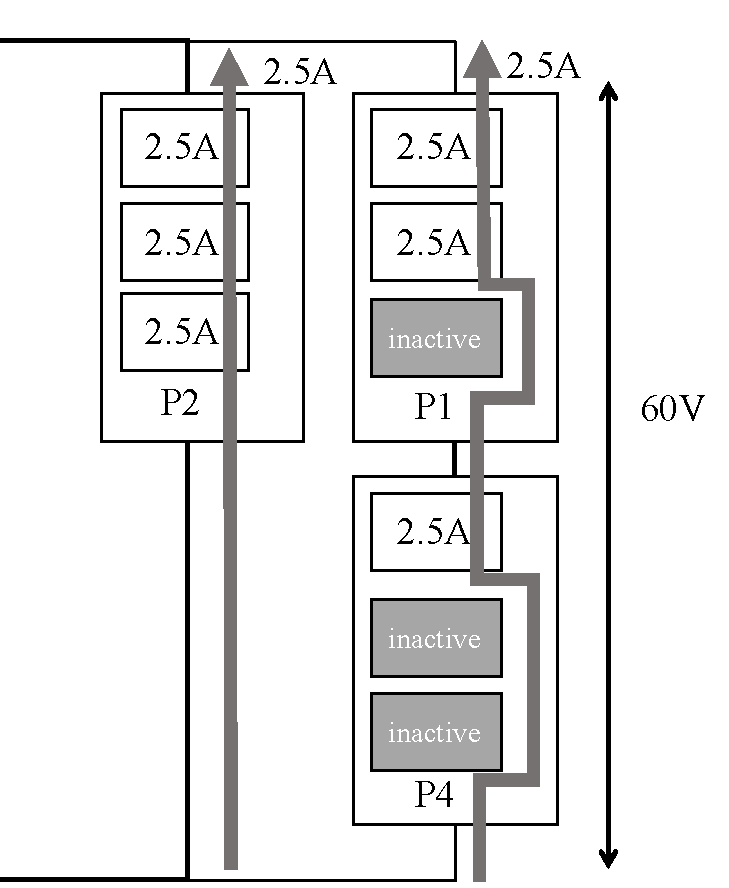
\includegraphics[width=0.5\linewidth]{fig/feasible-configuration.pdf}
    \caption{Feasible configuration}
    \label{fig:feasible-configuration}
\end{figure}

Now we will define the feasibility. For a PV array $A$ with $s$ strings, let $M_{A,i}(I)$ denote the number of modules that can be active with a current level $I$ in the $i$-th string.
Let $Q = (Q_{1},Q_{2},\ldots ,Q_{s})$ be a sequence of currents required for strings. 
A sequence of currents $Q$ is feasible with $m$ modules if and only if it is possible to form a PV array $A$ such that 
\begin{equation}
M_{A,i}(Q_{i}) \geq m
\end{equation}
holds for each string $i (1 \leq i \leq s)$.


%The definition of feasibility is in Equation \ref{feasibility}. When the number of working modules in a string ($M_S$) are less than the number of working module per-string ($Q_M$), this configuration is infeasible.
%\begin{equation}
%    \left\{\begin{matrix}
%        M_S < Q_{M} & & \text{Infeasible}\\ 
%        M_S \geqslant Q_{M} & & \text{Feasible} 
%    \end{matrix}\right.
%    \label{feasibility}
%\end{equation}
%
%For example, An 3X3 PV array formed by 9 PV panels. The number of modules that are able to work at current value for each string as showed in Table \ref{not_feasible}.The dot in each block in form of a PV module. As the number of modules and the panel they belong to, it is straight forward that panel P1 for any current value it have at least 2 modules can work. Instead of panel P9 only have 1 module can work at 0.5A.
%One configuration requires 6 modules working for each string at 0.5A, 0.5A and 3A($Q_M = 6$). According to Table \ref{not_feasible} there isn't any combination for such configuration. Of course we can compute it by using exhaustive searching. However it is time-consuming. So we need an algorithm to efficiently identify feasibility for each configuration candidates.

%\begin{table}[htbp]
%    \caption{Infeasible Example}
%    \begin{center}
%    \begin{tabular}{c|c|c|c|c|c|c|c|c|c}
%    \hline\hline
%             & P1 & P2  & P3  & P4 & P5 & P6  & P7  & P8  & P9  \\ \hline
%         0.5A & ***& *** & *   & *  & ***& **  & *   & *** & * \\ \hline
%         1.5A & ***& *** & *   & *  & ***&     & *   &     &   \\ \hline
%         3A   & ** & **  & *   & *  & ** &     &     &     &   \\\hline \hline
%    \end{tabular}
%    \label{not_feasible}
%    \end{center}
%\end{table}

\section{An algorithm to identify feasibility}\label{Sec5}
\subsection{Feasibility Problem}\label{Sec5_1}
In this section, we propose an algorithm to identify feasibility.
First we will formulate the feasibility problem that identify the feasibility for given current sequence and the number of active modules per string as follows.
\begin{definition}[Feasibility Problem]\\
Input: information of MPPs (approximated values), a current sequence $Q$, and the number $m$ of active modules per string.\\
Output: Whether $Q$ with $m$ modules is feasible or not.
\end{definition}

%The input of algorithm is the information of PV array and Configuration candidates. The information of PV array contains a set of panels and the number of working modules in each panel for each current values. Table \ref{Info_Array} shows the information of a PV panel from Table \ref{not_feasible} for configuration \{0.5A, 0.5A, 3A, $Q_M = 6$ \}.
%\begin{table}[htbp]
%    \caption{Information of PV Array}
%    \begin{center}
%    \begin{tabular}{c|c|c|c|c|c|c|c|c|c}
%    \hline\hline
%             & P1 & P2  & P3  & P4 & P5 & P6  & P7  & P8  & P9  \\ \hline
%         String1-0.5A & 3& 3 & 1   & 1  & 3& 2  & 1   & 3 & 1 \\ \hline
%         String2-0.5A & 3& 3 & 1   & 1  & 3& 2  & 1   & 3 & 1  \\ \hline
%         String3-3A   & 2 & 2  & 1   & 1  & 2 & 0  &0   &0  &0  \\\hline \hline
%    \end{tabular}
%    \label{Info_Array}
%    \end{center}
%\end{table}
%It terms that for panel P2, 3 modules are able to work on String1 or String2 and 2 modules are able to work on String3. Due to one panel can only connected to single string. So the output of algorithm is the feasibility answer for a configuration. That is, the algorithm determines whether there exists an assignment of panels to strings that realizes the configuration required.

\subsection{Outline of the algorithm}

In the proposed algorithm, we try to configure a PV array and identify the feasibility. For a given current sequence $Q = (Q_{1},Q_{2},\ldots ,Q_{s}) (Q_{i} \geq Q_{j} \mbox{\ if\ } i \leq j)$, we will assign panels to strings in the order of $Q_{1},Q_{2},\ldots ,Q_{s}$. When selecting a panel to a string, we will consider how much we lose an opportunity that the panel is more effectively used for other current level. For example, if we select Panel 1 in Table \ref{tab:modules} for a string with a current level 3A, two modules can be active while the remaining one module becomes inactive. 
The remaining one module still is not active if $P1$ is used for a current level 2,5A, while it can be active if it is used for current level 1.5A or 0.5A. We will consider that when selecting $P1$ for a current level 3A, we don't have any loss for a current level 2.5A but lose one module for 1.5A and 0.5A. The algorithm select panels so as to minimize such losses. 

Let $M_{p}(I)$ denote the number of modules that can be active at current level $I$ in a PV panel $p$. 
For a given current sequence $Q = (Q_{1},Q_{2},\ldots ,Q_{s}) (Q_{i} \geq Q_{j} \mbox{\ if\ } i \leq j)$, 
a loss of selecting a panel $p$ at the $k-1$-th string for the $k$-th string is defined as 
$Loss(p,k) = M_{p}(Q_{k}) - M_{p}(Q_{k-1})$. 

%
%Let the $S$ for the number of PV strings and $P$ be the number of PV panels, $M_{(i,p)}$ is the number of modules on panel $p$ at current value $i$. For each panel we consider the different vector $Loss[p,k] = M_{(i_{k-1},p)}-M_{(i_{k},p)} ,(k \leq S)$. This vector means if we use panel $p$ on current $k$  it will loss $Loss[p,k]$ working modules in current $k-1$. Without loss of generality, for each panel $p$, $Loss^*[p] = ( Loss[p,k_1], Loss[p,k_2],..., Loss[p,k_S] )$ and $Loss^*[p_i] \leq Loss^*[p_j]$ holds for any $i \leq j$. After sorting all panels in lexicographic order by vector $Loss^*[p]$, we will have a order for arranging panels in different location.

To assign panels for the $n$-th string, the following steps are applied. Let $m$ be the required number of active modules.
\begin{enumerate}
\item Sort unselected PV panels in a lexicographically ascending order of $Loss(p,n+1)$, $Loss(p,n+2)$,$\ldots$, $Loss(p,s)$ and $M_{p}(Q_{n})$.
\item Select PV panels until selecting $m$ or more active modules for a current level $Q_{n}$.
\item Cancel redundant PV panels so that the number of active modules at a current level $Q_{n}$ is minimized.
\item Swap selected PV panels with unselected PV panels so that the number of selected PV panels is minimized.
\end{enumerate}

Before explaining more details, we first show an example. Table \ref{tab:proposed-example} shows how to select PV panels for the first string where the required number $m$ of active modules is 5. 
Panels are sorted by $Loss$ and $M_{p}(Q_{1})$ (the number of active modules for the first string) in the order of $P1$, $P2$, $\ldots$, $P7$. 
In the example, panels $P2$ to $P6$ are at the same loss level $(1,0)$. 
PV panels are selected for each loss level. First, $P1$ is selected, then panels at the second loss level are selected in the order of $P2$, $P3$, $\ldots$. After selecting until $P5$, the number of active modules exceed $m (=5)$. In this case, if there is some redundant panels, these panels are canceled. In the example, $P4$ is canceled. Finally, if some of selected PV panels can be swapped with less number of unselected panels, they are swapped. In the example, $P2$ and $P3$ are swapped with $P6$. Consequently, three panels $P1$, $P5$ and $P6$ are selected. 

\begin{table}[t]
\caption{An example of the proposed method ($m = 5$)}
\begin{center}
\begin{tabular}{c|c|ccccc|c}\hline \hline
                               & \multicolumn{7}{c}{Panels}  \\
                               &  \multicolumn{1}{c}{$P1$}    & $P2$   & $P3$    & $P4$    & $P5$   & \multicolumn{1}{c}{$P6$}            & $P7$             \\ \hline
$M_{p}(Q_1)$        & 1     & 1     & 1     & 1     & 2    & 2    & 2              \\ \hline
$M_{p}(Q_2)$        & 1     & 2     & 2     & 2     & 3    & 3    & 2              \\ \hline
$M_{p}(Q_3)$        & 1     & 2     & 2     & 2     & 3    & 3    & 3              \\ \hline
$Loss(p,2)$           & 0     & 1     & 1     & 1     & 1    & 1    & 1    \\ \hline
$Loss(p,3)$           & 0     & 0     & 0     & 0     & 0    & 0    & 1    \\ \hline\hline
step 2        & $\surd$ & $\surd$ &$\surd$ &$\surd$ &$\surd$ & & \\ \hline
step 3      & $\surd$ & $\surd$ &$\surd$ & &$\surd$ & & \\ \hline
step 4       & $\surd$ &  & & &$\surd$ & $\surd$ & \\ \hline         
\end{tabular}
\end{center}
\label{tab:proposed-example}
\end{table}

\subsection{Algorithm}
Step 1 sorts unselected panels (with modules that can be active for the target current), and Step 2 selects panels one by one in the sorted order until reaching the required number of active modules.  

Step 3 optimizes the number of active modules. 
In Step 3, if the number of active modules exceeds the required number $m$, redundant panels are canceled if exist. 
A panel is \textit{redundant} if the number of active modules is still $m$ or more even if the panel is canceled.  
Redundant panels are searched at loss level. 
Starting with a loss level where the last panel is selected, we will check the number of active modules $M_{p}(Q_{n})$ for each panel $p$ 
where $Q_{n}$ is a required current level for the current string.
Redundant panels are selected and canceled from panels with less number of $M_{p}(Q_{n})$ in the same loss level. 
If there still exceed $m$ after canceling, we will go to the previous loss level and try to cancel panels.
This procedure is repeated until selecting an exact $m$ active modules or checking all the loss levels.

Step 4 optimizes the number of selected panels.
In Step 4, we will swap selected panels and an unselected panel in the same loss level to reduce the number of selected panels.
There are 3 swap cases as shown in Table \ref{tab:swap}. Algorithm 1 shows a pseudo code of the proposed algorithm.



\begin{table}[t]
\caption{Swap rule}
\label{tab:swap}
\centering
\begin{tabular}{c|c}
\hline\hline
\multicolumn{2}{c}{The numbers of active modules} \\
selected panels & unselected panels \\ \hline
1, 1, 1 & 3 \\ \hline
1, 1 & 2 \\ \hline
1, 2 & 3 \\ \hline
\end{tabular}
\end{table}




%To assign panels in right location, following steps are required.
%\begin{enumerate}[(1)]
%\item Selecting panel from sorted panels until selected contain enough PV modules working at the highest desired current value.
%\item Remove selected panels which don't have PV modules working at the highest desired current value for further more selection.
%\item In selected panels, try to find a combination that provided exact number of modules working at the highest desired current value.\label{find_exact}
%\item Swap selected panels to find a combination with minimum number of panels. This SWAP will follow several priorities.\label{swap}
%\item If SWAP approved, step \ref{swap} will be repeated till number of panels are minimized.
%\item Otherwise, none of SWAP will be approved. Evaluate selected panels with feasibility requirement in \ref{Sec4} equation (\ref{feasibility}).
%\item If there remain any un-selected panel, as them to different PV strings that balance the string length.
%\end{enumerate}

%We explain step (\ref{find_exact}) and (\ref{swap}) that finding a local optimized combination of a desired current value. To do this, we begin with sorting panels by vector $Loss^*[p]$. That will let a panel with minimum module losses be the first one in a string with highest current value. When $Loss^*[p_a] = Loss^*[p_b]$ which means panel $a$ and panel $b$'s module losses are same and they are in same loss level ($LV$). By using vector $LV$ we can divide selected panels into different groups.
%
%To get exact number of working modules, we start to search panels form last loss level to first loss level. In each $LV$ remove the panel $x$ which $M_{(j,x)} \leq Q_M - \sum (M_{(j,\textup{Selected Panels})})$. This step will cut the number of panels and increase flexibility.


%\begin{table}[htbp]
%\caption{SWAP Example}
%\begin{center}
%\begin{tabular}{c|ccccc|cc}\hline \hline
%                               & \multicolumn{5}{c|}{Selected Panels} & \multicolumn{2}{c}{Swap Panels} \\
%                               & $P1$    & $P2$   & $P3$    & $P4$    & $P5$   & $P6$            & $P7$             \\ \hline
%High                           & 1     & 1     & 1     & 1     & 2    & 2              & 2              \\ \hline
%Low                            & 1     & 1     & 1     & 2     & 3    & 3              & 3              \\ \hline
%$Loss^*[p]$ & 0     & 0     & 0     & 1     & 1    & 1              & 1             
%\end{tabular}
%\end{center}
%\label{table_swap}
%\end{table}

%For swapping panels, panels with same $LV$ as selected panels can be swapped. In order to not loss flexibility, swapped panles' $Loss^*[p]$ should less than unswap panels'. For example as Table \ref{table_swap}, panel $P1-P5$ are selected panels. Panel $P6$ and $P7$ have the same $Loss^*[p]$ vector as $P5$, so they are able to swap. Due to $P1$ and $P2$'s $Loss^*[p]$ are less than $P6$'s, we can not swap them. On the other hand, we can swap panel $P1$ and $P4$ with $P6$. Keeping the same module losses and further reduce the number of panels.  Pseudo codes are given below to give details to summarize the process of proposed algorithm.

\begin{algorithm}
\caption{Feasibility Check}
\LinesNumbered
\SetKwInOut{Input}{Input}  
\Input{
  \textit{$Q = Q_1, Q_2, \ldots , Q_s$}: required current for each string; 
  \textit{$m$}: The minimum number of active modules per string;
  \textit{$M_{p}$}: The number of active modules in each panel \textit{p};
  %\textit{P}: Number of panels; 
  \textit{s}: Number of strings;}
\SetKwInOut{Output}{Output}
\Output{Feasibility Result;%\\
        %Conf: Configuration Result;
        }
\For{\textup{each string} $ k (2 \leq k \leq s)$ \textup{and panel} $p$}{$Loss(p,k) = M_{p}(Q_{k}) - M_{p}(Q_{k-1})$}
\For{j = 1 to s}
    {{\If{$\sum M_{p}(Q_{j})$ \textup{for unselected panes} $< m$}
       {\textup{\textbf{return :}} Feasibility = NO}}
     $PS$ = a set of unselected panels with $M_{p}(Q_{j}) > 0$;\\
     // step 1\\
     sort $PS$ in a lexicographically ascending order of $Loss(p,j+1)$, $Loss(p,j+2)$, $\ldots$, $Loss(p,s)$, $M_{p}(Q_{j})$;\\
     // step 2\\
     select panels in the order in $PS$ until $\sum M_{p}(Q_{j})$ for selected panels $\geq m$;\\
     //step 3\\
     group selected panels $LV_{1}$, $LV_{2}$,$\ldots$, $LV_{h}$ with loss level ($LV_{1}$ is the lowest level);\\
     \For{i = h to 1}
     {find and cancel redundant panels in $LV_{i}$ in the order in $PS$}
     //step 4\\
     \For{i = h to 1}
     {apply swap rules for selected panels in $LV_{i}$ and an unselected panel in the same loss level}
    }
    \textup{\textbf{return :}} Feasibility = YES
\end{algorithm}

%\begin{algorithm}
%    \caption{find exact \# of modules}
%    \LinesNumbered
%    \KwIn{$TempConf$, n, $Loss^*[p]$,Over}
%    \KwOut{Conf[j]}
%    $i$ = $h$ = 1; $LV[h]$ = \{$p_{\alpha_1}$\};\\
%    \While{i $\neq$ $\left|PSet\right|$}
%        {i++;\\
%        \uIf{$Loss^*[p_{\alpha_i}]$ == $Loss^*[p_{\alpha_{i-1}}]$}
%            {$LV[h] = LV[h]$ $\cup$ \{$p_{\alpha_i}$\}\\
%            \textup{\textbf{continue;}}}
%        \uElseIf{i $>$ n}
%            {\textup{\textbf{break;}}}
%        \Else{h++;\\$LV[h]$ = \{$p_{\alpha_i}$\}}
%    }
%    \While{h$\neq$0}
%        {\eIf{Over == 0}
%            {\textbf{\textup{break;}}}
%        {L=$\left|\{p_i \in LV^*[h^{'}]\mid h^{'} \leq h-1 \}\right|$\\
%        $l^{*} = \left|\{p_i \in LV^*[h]\mid M_{(j,\alpha_i)} \leq Over \}\right|$\\
%        Let $l$ be the minimum index $l^{'}$ such that $\sum^{l^{*}}_{t=l^{'}}M_{(j,\alpha_{L+t})}\leq Over$\\
%        $Over = Over - \sum^{l^{*}}_{t=l^{'}}M_{(j,\alpha_{L+t})}$;\\
%        $TempConf$ = $TempConf$ - $\{p_{L+l}, p_{L+l+1},..., p_{L+l^*}\}$;\\
%        $h- -$;}
%    }
%    $U = \{p_{\alpha_{1}}, p_{\alpha_{2}},..., p_{\alpha_{i-1}}\}$;\\
%    $N = U-TempConf$;\\
%    \Repeat{x==$\left|N\right|$}
%        {Let $\beta_1, \beta_2, \beta_3,...,\beta_{\left|TempConf\right|}$ be new indices of $TempConf$;\\
%        Let $\gamma_1, \gamma_2, \gamma_3,...,\gamma_{\left|N\right|}$ be new indices of $N$;\\
%        \For{x = 1 to $\left|N\right|$}
%            {\ForAll{$p_\beta$ in $TempConf$}
%                {\uIf{$\sum M_{(j,\beta}$==$M_{(j,\gamma_x)}$}
%                    {$TempConf = TempConf - \{p_{\beta}\}+\{p_{\gamma_x}\}$;\\
%            % $N^* = \left|N\right|$\\
%            $N = N - \{p_{\gamma_x}\}$;\\
%            \textbf{\textup{Continue;}}\\}}}
%        }
%\end{algorithm}

%\begin{algorithm}
%\caption{Sort panel by lexicographic order}
%\LinesNumbered
%\SetKwInOut{Input}{Input}  
%\Input{\textit{$M_{(i,p)}$}: The number of modules in panel \textit{p} at current \textit{i};
%  \textit{P}: Number of panels; \textit{S}: Number of strings;
%  \textit{$Q_M$}: The minimum number of modules for each string;}
%\SetKwInOut{Output}{Output}
%\Output{Feasibility Result;\\
%        Conf: Configuration Result;}
%\For{k = 1 to S-1, \textup{\textbf{each}} panel $p$}{$Loss[p,k] = M_{(i_{S-k},p)}-M_{(i_{S-k+1},p)}$}
%PSet = $\{p_1, p_2,...,p_P\}$\\
%\For{j = S to 1}
%    {n = 1;\\
%     \For{\textup{\textbf{each}} p $\in$ PSet}
%        {$Loss^*[p] = (Loss[p,S-j+1], Loss[p,S-j+2],..., Loss[p,S])$\\
%        Let $\alpha_1, \alpha_2,..., \alpha_{|PSet|}$ be indices such that $Loss^*[p_{\alpha i}] \leq Loss^*[p_{\alpha j}]$ holds for $ \textup{\textbf{any}}$ i $\leq$ j\\
%        \tcc{Sort Panels in lexicographical order by \textit{Loss}}}
%     \While{\textup{SUM} = $\sum_{k=1}^{n} M_{(i_j,\alpha_k)} < Q_M$}
%        {\If{n == $PSet$}
%            {\textup{\textbf{return :}} Feasibility = NO}n++;\\}
%        $TempConf$ = \{ $p_{\alpha_1}$, $p_{\alpha_2}$, $p_{\alpha_3}$,..., $p_{\alpha_n}$ \};\\
%    \ForAll{panels in $TempConf$}
%        {remove panels which $M_{(j,\alpha)} == 0$}
%    %  \For{m = 1 to n}
%    %     {\If{$M_{(j,\alpha_m)} == 0$}
%    %         {$TempConf$ = $TempConf$ -\{$p_{\alpha_m}$\}}}
%    %  \eIf{SUM == $Q_M$ \textup{or} j == 1}
%    %     {Conf[j] = $TempConf$}
%    %     {Over = SUM - $Q_M$;\\\textup{\textbf{Do} Algorithm 2}}
%        Over = SUM - $Q_M$;\\\textup{\textbf{Do} Algorithm 2}\\
%        % Conf[j] = $TempConf$\\
%        $PSet$ = $PSet$ - Conf[j];\\
%    }
%    \textup{\textbf{return :}} Feasibility = YES
%\end{algorithm}
%
%\begin{algorithm}
%    \caption{find exact \# of modules}
%    \LinesNumbered
%    \KwIn{$TempConf$, n, $Loss^*[p]$,Over}
%    \KwOut{Conf[j]}
%    $i$ = $h$ = 1; $LV[h]$ = \{$p_{\alpha_1}$\};\\
%    \While{i $\neq$ $\left|PSet\right|$}
%        {i++;\\
%        \uIf{$Loss^*[p_{\alpha_i}]$ == $Loss^*[p_{\alpha_{i-1}}]$}
%            {$LV[h] = LV[h]$ $\cup$ \{$p_{\alpha_i}$\}\\
%            \textup{\textbf{continue;}}}
%        \uElseIf{i $>$ n}
%            {\textup{\textbf{break;}}}
%        \Else{h++;\\$LV[h]$ = \{$p_{\alpha_i}$\}}
%    }
%    \While{h$\neq$0}
%        {\eIf{Over == 0}
%            {\textbf{\textup{break;}}}
%        {L=$\left|\{p_i \in LV^*[h^{'}]\mid h^{'} \leq h-1 \}\right|$\\
%        $l^{*} = \left|\{p_i \in LV^*[h]\mid M_{(j,\alpha_i)} \leq Over \}\right|$\\
%        Let $l$ be the minimum index $l^{'}$ such that $\sum^{l^{*}}_{t=l^{'}}M_{(j,\alpha_{L+t})}\leq Over$\\
%        $Over = Over - \sum^{l^{*}}_{t=l^{'}}M_{(j,\alpha_{L+t})}$;\\
%        $TempConf$ = $TempConf$ - $\{p_{L+l}, p_{L+l+1},..., p_{L+l^*}\}$;\\
%        $h- -$;}
%    }
%    $U = \{p_{\alpha_{1}}, p_{\alpha_{2}},..., p_{\alpha_{i-1}}\}$;\\
%    $N = U-TempConf$;\\
%    \Repeat{x==$\left|N\right|$}
%        {Let $\beta_1, \beta_2, \beta_3,...,\beta_{\left|TempConf\right|}$ be new indices of $TempConf$;\\
%        Let $\gamma_1, \gamma_2, \gamma_3,...,\gamma_{\left|N\right|}$ be new indices of $N$;\\
%        \For{x = 1 to $\left|N\right|$}
%            {\ForAll{$p_\beta$ in $TempConf$}
%                {\uIf{$\sum M_{(j,\beta}$==$M_{(j,\gamma_x)}$}
%                    {$TempConf = TempConf - \{p_{\beta}\}+\{p_{\gamma_x}\}$;\\
%            % $N^* = \left|N\right|$\\
%            $N = N - \{p_{\gamma_x}\}$;\\
%            \textbf{\textup{Continue;}}\\}}}
%        }
%\end{algorithm}

\subsection{Evaluation}
Although the pilot example refers to three strings only, the extension of the method to any number of parallel connected strings is the same.

To evaluate the performance of proposed algorithm, we compare the result with exhaustive searching algorithm for 100 random shadow distributed PV array. For each PV array, contains 
6 - 24
% {\color{red} \textbf{how many - how many}} 
PV panels connected into 
3 - 6
% {\color{red} \textbf{how many - how many}} 
PV strings. For each PV panels, it will have 
3 - 8
% {\color{red}{how many - how many}} 
working current value.

The computational time required for finding optimal configuration and accuracy of feasibility judgment in the proposed algorithm and exhaustive search algorithm are compared in Table \ref{result_compare}. As shown in Table \ref{result_compare}, proposed algorithm achieved less computing time compare with exhaustive search algorithm and with high accuracy.  

\begin{table}[htbp]
\caption{}
\begin{center}
\begin{tabular}{ccc}
\multicolumn{3}{c}{\begin{tabular}[c]{@{}c@{}}COMPARISON BETWEEN EXISTED METHODS\\ AND PROPOSED ALGORITHM\end{tabular}}                                         \\ \hline \hline
\multicolumn{1}{c|}{}                         & \multicolumn{1}{c|}{Proposed Algorithm} & \begin{tabular}[c]{@{}c@{}}Exhaustive search \\ Algorithm\end{tabular} \\ \hline
\multicolumn{1}{c|}{Number of PV Array}       & \multicolumn{2}{c}{-}                                                                                         \\ \hline
\multicolumn{1}{c|}{Number of MPP candidates} & \multicolumn{2}{c}{-}                                                                                       \\ \hline
\multicolumn{1}{c|}{Feasible Candidates}      & \multicolumn{1}{c|}{-}              & -                                                                   \\ \hline
\multicolumn{1}{c|}{Infeasible Candidates}    & \multicolumn{1}{c|}{-}              & -                                                                   \\ \hline
\multicolumn{1}{c|}{Error Rate}               & \multicolumn{1}{c|}{0.89\%}            & 0\%                                                                    \\ \hline
\multicolumn{1}{c|}{Ave. times per Array}     & \multicolumn{1}{c|}{0.157s}            & 4370s                                                                 
\end{tabular}
\label{result_compare}
\end{center}
\end{table}

% \section{Simulation}\label{Sec6}
% In this section, we consider using 3 different size PV array, which are 3 $\times$ 4 array, 60 $\times$ 4 array and 40 $\times$ 15 array. The whole process though SPICE simulation with the configuration result by proposed algorithm. The PV cell's parameters are shown in Table \ref{PV_cell_par}.

% \begin{table}[]
% \caption{PV Cell Parameters}
% \begin{center}
% \begin{tabular}{c|c}
% \hline \hline
% Parameter             & Value  \\ \hline
% Short-Circuit Current & 0.66A  \\
% MPP-Current           & 0.58A  \\
% Open-Circuit Voltage  & 280V   \\
% MPP-Voltage           & 215V  \\
% Max Power Output      & 124.7W 
% \end{tabular}
% \end{center}
% \label{PV_cell_par}
% \end{table}
% \subsection{3 $\times$ 4 Array}
% In a 3 $\times$ 4 array, there are 12 panels connected in parallel for 4 strings, for each string contains 3 PV panels. The shadow conditions for PV array are not uniformly, as shown in Fig. \ref{shadow_3x4_a}. Without reconfiguration, PV array output I-V characteristic as shown in Fig. \ref{shadow_3x4_b}. The global MPP as {\color{red}{how many Watt}} on {\color{red}{how many voltage}}. After proposed algorithm based reconfiguration, this PV array achieved {\color{red}{how many Watt}} on {\color{red}{how many voltage}} for global MPP. The output power has increased by {\color{red}{how many \%}}
% \subsection{60 $\times$ 4 Array}
% For medium size 60 $\times$ 4 array, on standard test condition the power output are {\color{red}{how many KW}} without any shadow. Fig. \ref{shadow_60x4_a} presents the shadow distribution amount the PV array which power output are {\color{red}{how may KW}}. After reconfiguration, panel arrangement as illustrated in Fig. \ref{shadow_60x4_b}. With reconfiguration, power generation increased by {\color{red}{how many \%}}.
% \subsection{40 $\times$ 15 Array}
% As a large scale PV array. Although the algorithm proposed in \cite{orozco2016optimized} are hard to converge when the configuration candidates are widely distributed. The algorithm we proposed still calculate the feasible configuration result very fast. {\color{red}{60}} configuration candidates though the feasibility judgment algorithm in 269.6s with {\color{red}{20}} feasible configuration as shown in Table \ref{shadow_40x15_table}.
\section{Conclusions}\label{Sec7}

\section*{Acknowledgment}


% \section*{References}

\renewcommand\refname{Reference}
\bibliographystyle{ieeetr}
\bibliography{reference}

\end{document}
